\documentclass[pdflatex,compress,mathserif]{beamer}

%\usetheme[dark,framenumber,totalframenumber]{ElektroITK}
\usetheme[darktitle,framenumber,totalframenumber]{ElektroITK}

\usepackage[utf8]{inputenc}
\usepackage[T1]{fontenc}
\usepackage{lmodern}
\usepackage[bahasai]{babel}
\usepackage{amsmath}
\usepackage{amsfonts}
\usepackage{amssymb}
\usepackage{graphicx}
\usepackage{multicol}
\usepackage{lipsum}
\usefonttheme[onlymath]{serif}

\newcommand*{\Scale}[2][4]{\scalebox{#1}{$#2$}}%

\setbeamertemplate{caption}[numbered]

\title{MATEMATIKA DASAR}
\subtitle{Pertidaksamaan}

\author{Mifta Nur Farid}

\begin{document}

\maketitle

\section{Pertidaksamaan}

\begin{frame}
	\frametitle{Pertidaksamaan}
	\begin{itemize}
		\item Salah satu bentuk pertidaksamaan:
		$$ 2x+3 \leq 9 $$
		\item Beberapa nilai $x$ yang memenuhi dan yang tidak memenuhi pertidaksamaan
		\begin{center}
			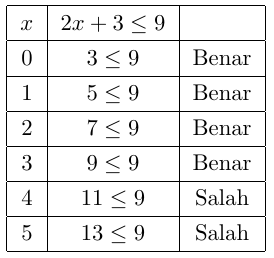
\includegraphics[width=0.4\linewidth]{img/img01}
		\end{center}
	\end{itemize}
\end{frame}

\begin{frame}
	\frametitle{Pertidaksamaan}
	\begin{itemize}
		\item Dalam persamaan $$ 2x+3 = 9 $$ memiliki solusi $x = 3$. Dalam garis bilangan:
		\begin{center}
			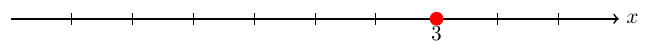
\includegraphics[width=\linewidth]{img/img02}
		\end{center}
		\item Dalam pertidaksamaan $$ 2x+3 \leq 9 $$ memiliki solusi $x \leq 3$. Dalam garis bilangan:
		\begin{center}
			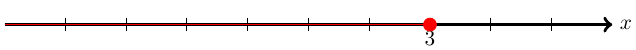
\includegraphics[width=\linewidth]{img/img03}
		\end{center}
	\end{itemize}
\end{frame}

\begin{frame}
	\frametitle{Pertidaksamaan}
	\begin{itemize}
		\item Dalam menyelesaikan pertidaksamaan dapat digunakan sifat-sifat berikut:
	\end{itemize}
	\begin{center}
		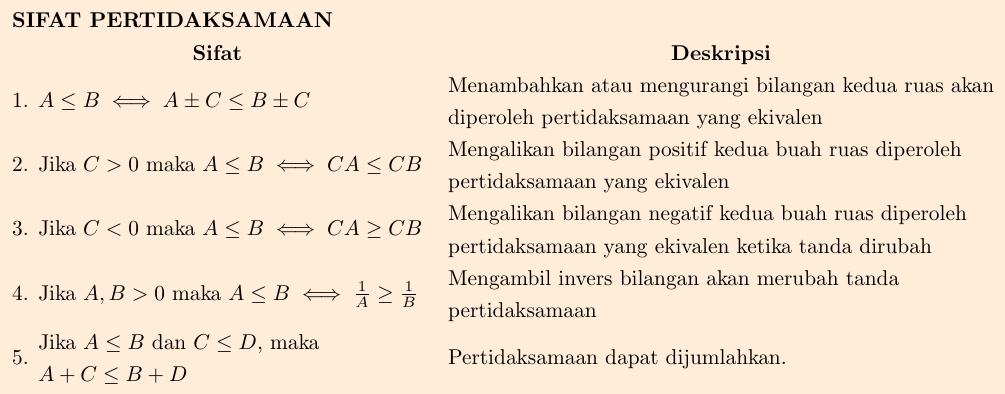
\includegraphics[width=\linewidth]{img/img04}
	\end{center}
\end{frame}

\section{Solusi Pertidaksamaan Linear}

\begin{frame}
	\frametitle{Solusi Pertidaksamaan Linear}
	\begin{center}
		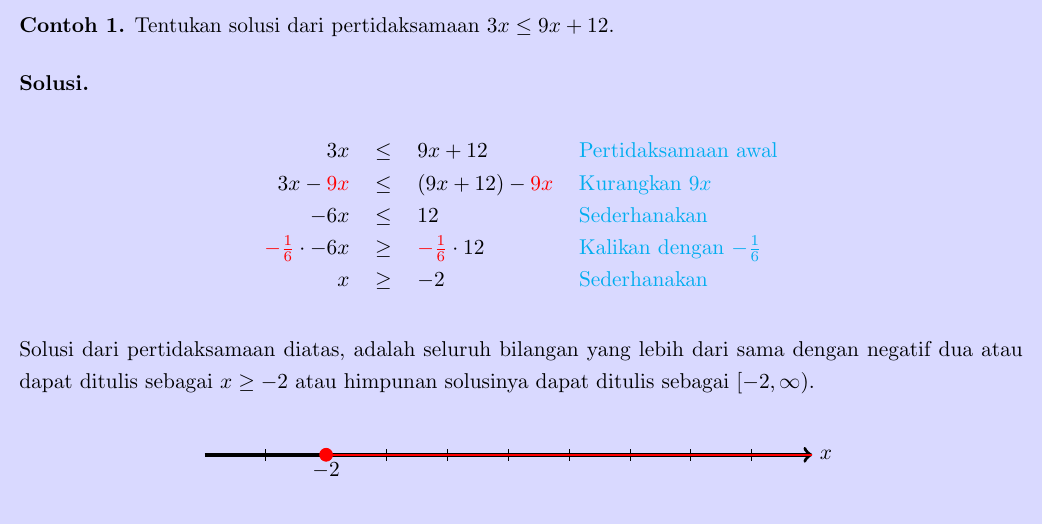
\includegraphics[width=\linewidth]{img/img05}
	\end{center}	
\end{frame}

\begin{frame}
	\frametitle{Solusi Pertidaksamaan Linear}
	\begin{center}
		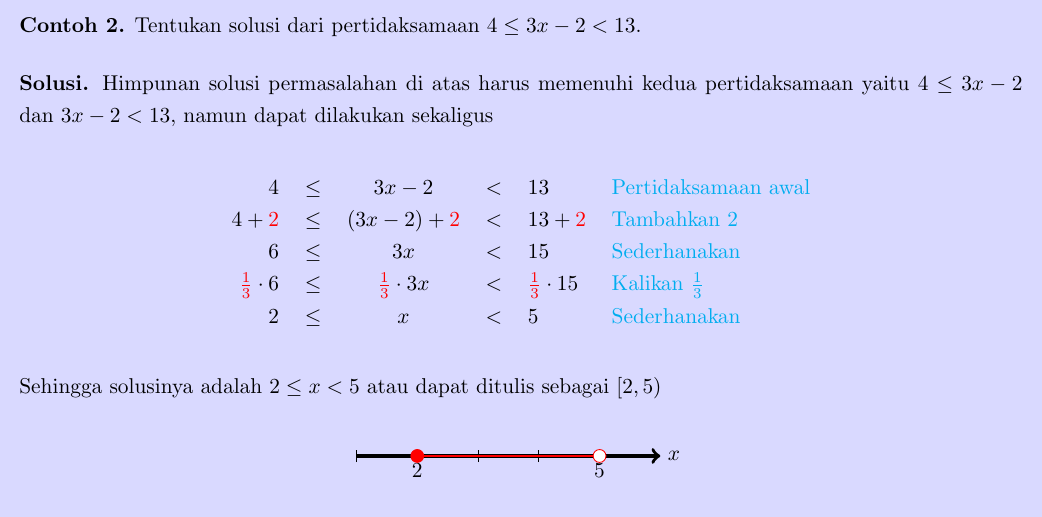
\includegraphics[width=\linewidth]{img/img06}
	\end{center}
\end{frame}


\section{Solusi Pertidaksamaan Tak Linear}

\begin{frame}
	\frametitle{Solusi Pertidaksamaan Tak Linear}
	\begin{center}
		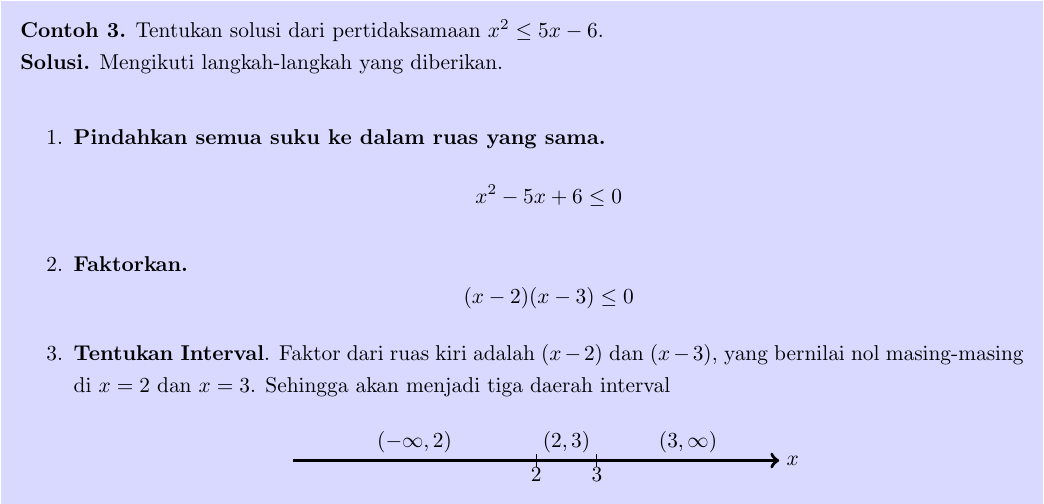
\includegraphics[width=\linewidth]{img/img07}
	\end{center}
\end{frame}

\begin{frame}
	\frametitle{Solusi Pertidaksamaan Tak Linear}
	\begin{center}
		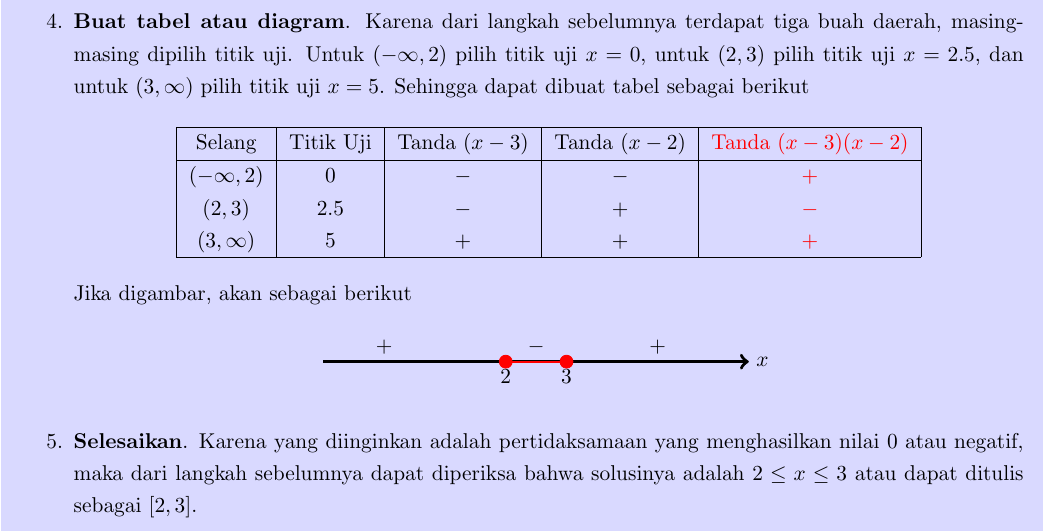
\includegraphics[width=\linewidth]{img/img08}
	\end{center}
\end{frame}

\begin{frame}
	\frametitle{Solusi Pertidaksamaan Tak Linear}
	\begin{center}
		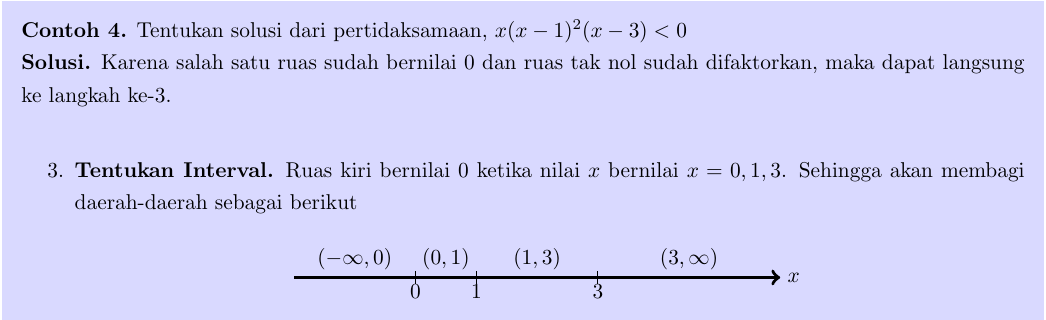
\includegraphics[width=\linewidth]{img/img09}
	\end{center}
\end{frame}

\begin{frame}
	\frametitle{Solusi Pertidaksamaan Tak Linear}
	\begin{center}
		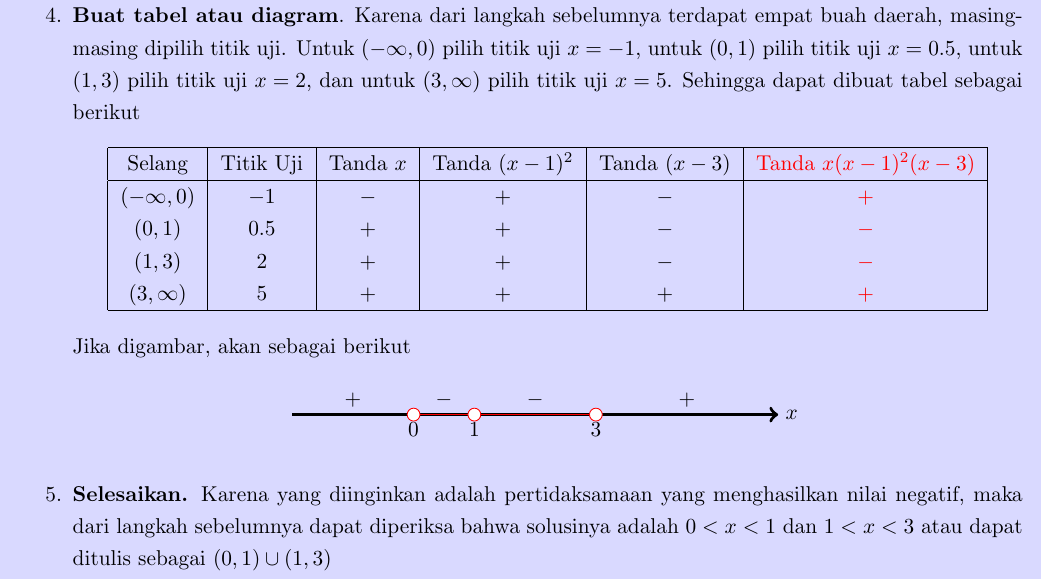
\includegraphics[width=\linewidth]{img/img10}
	\end{center}
\end{frame}

\begin{frame}
	\frametitle{Solusi Pertidaksamaan Tak Linear}
	\begin{center}
		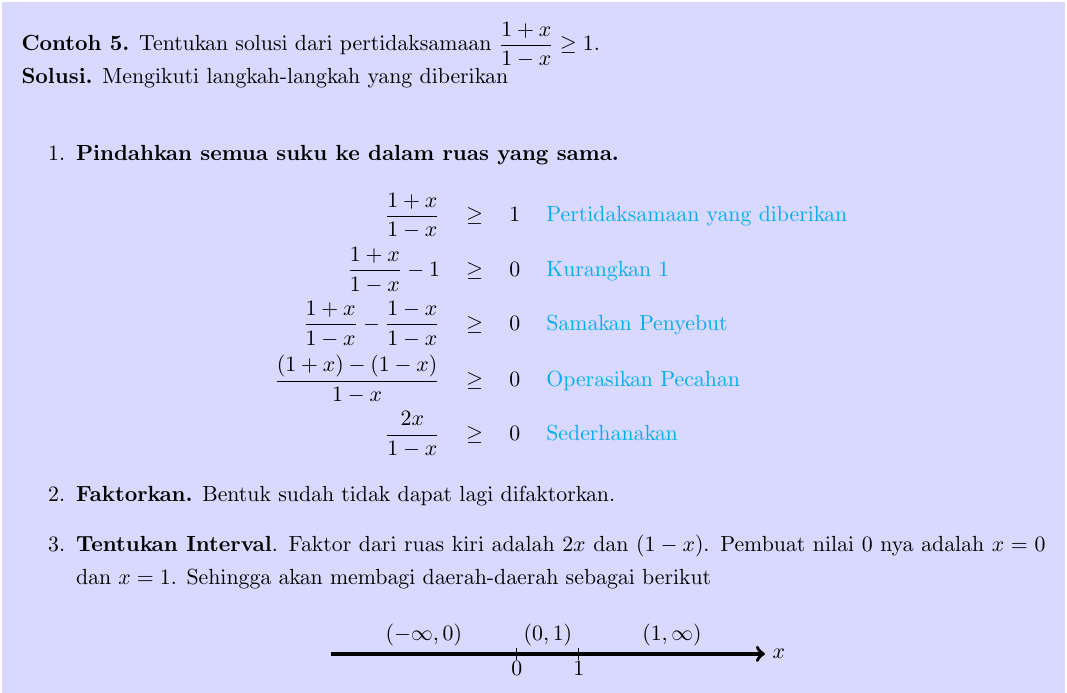
\includegraphics[width=\linewidth]{img/img11}
	\end{center}
\end{frame}

\begin{frame}
	\frametitle{Solusi Pertidaksamaan Tak Linear}
	\begin{center}
		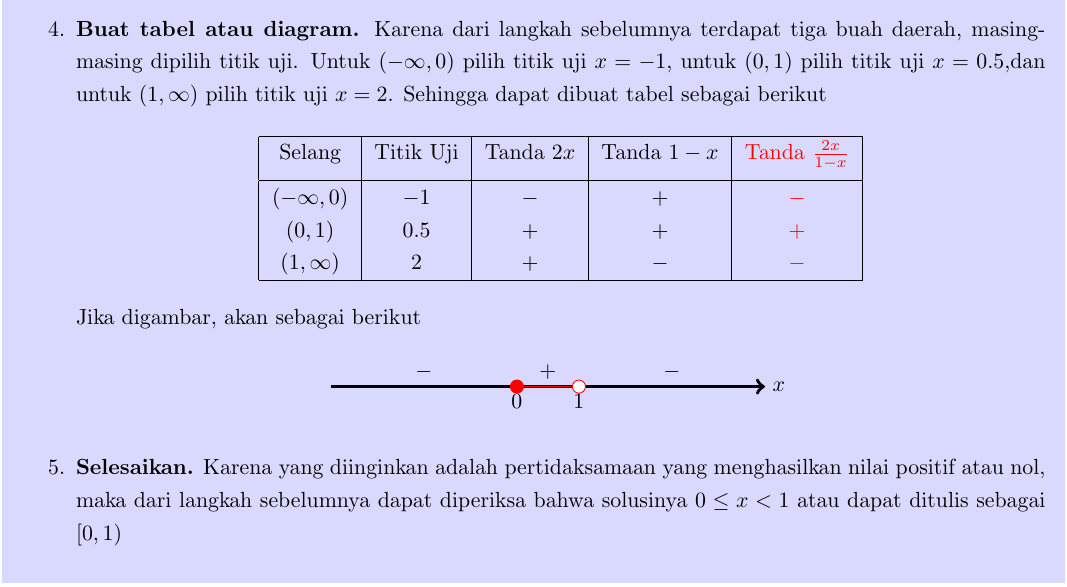
\includegraphics[width=\linewidth]{img/img12}
	\end{center}
\end{frame}

\section{Permodelan Masalah dengan Pertidaksamaan}

\begin{frame}
	\frametitle{Solusi Pertidaksamaan Tak Linear}
	\begin{center}
		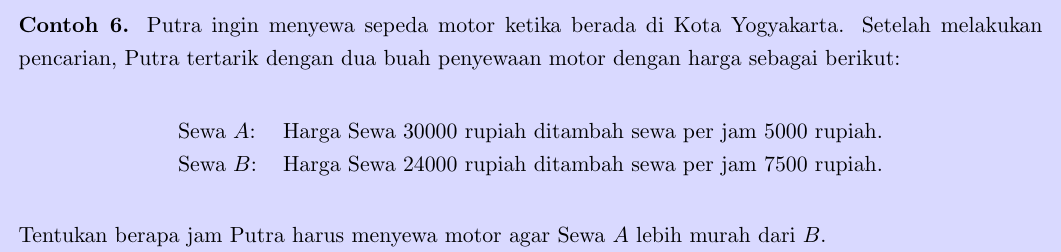
\includegraphics[width=\linewidth]{img/img13}
	\end{center}
\end{frame}

\begin{frame}
	\frametitle{Solusi Pertidaksamaan Tak Linear}
	\begin{center}
		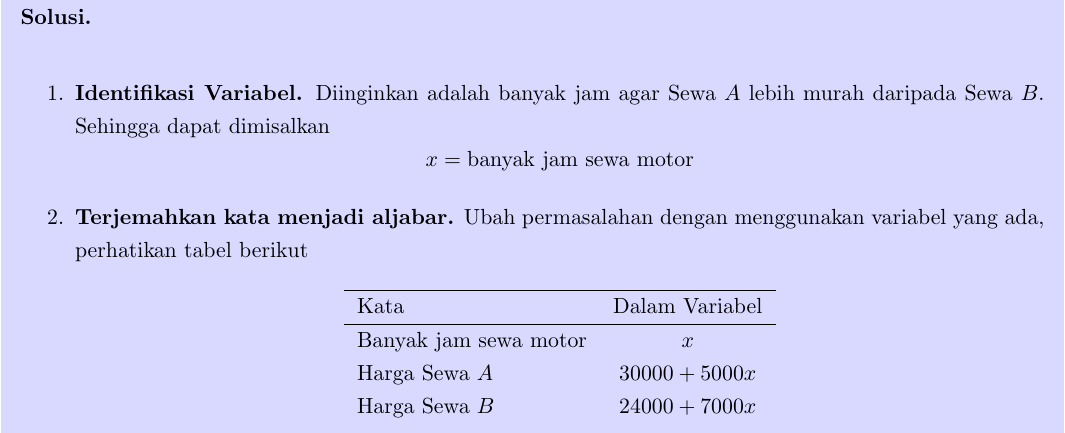
\includegraphics[width=\linewidth]{img/img14}
	\end{center}
\end{frame}

\begin{frame}
	\frametitle{Solusi Pertidaksamaan Tak Linear}
	\begin{center}
		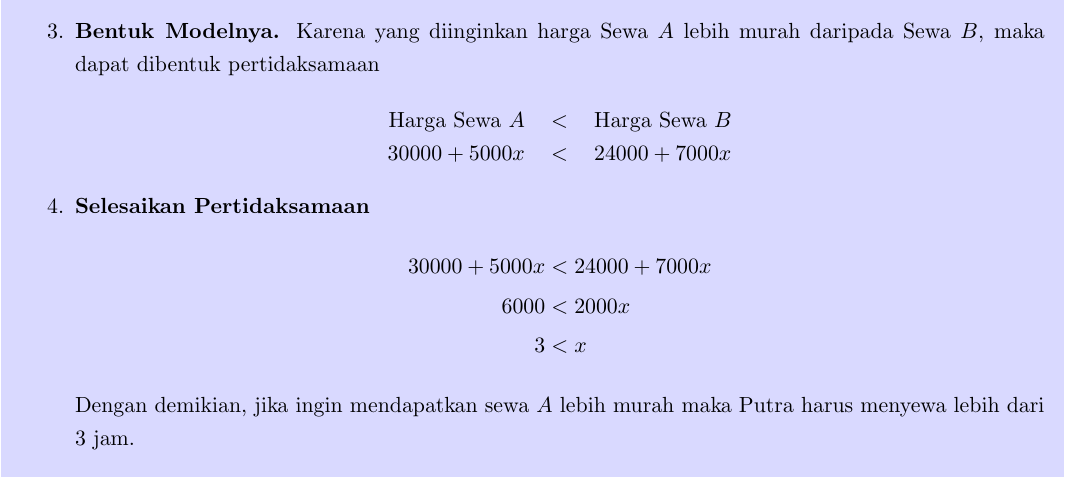
\includegraphics[width=\linewidth]{img/img15}
	\end{center}
\end{frame}

\begin{frame}
	\frametitle{Solusi Pertidaksamaan Tak Linear}
	\begin{center}
		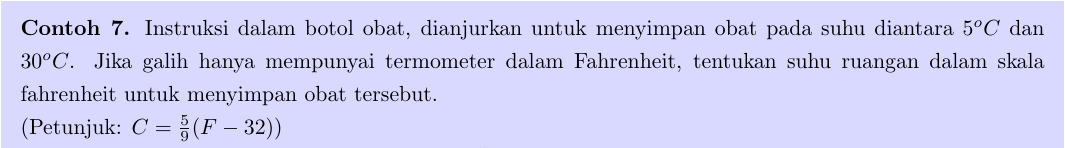
\includegraphics[width=\linewidth]{img/img16}
	\end{center}
\end{frame}

\begin{frame}
	\frametitle{Solusi Pertidaksamaan Tak Linear}
	\begin{center}
		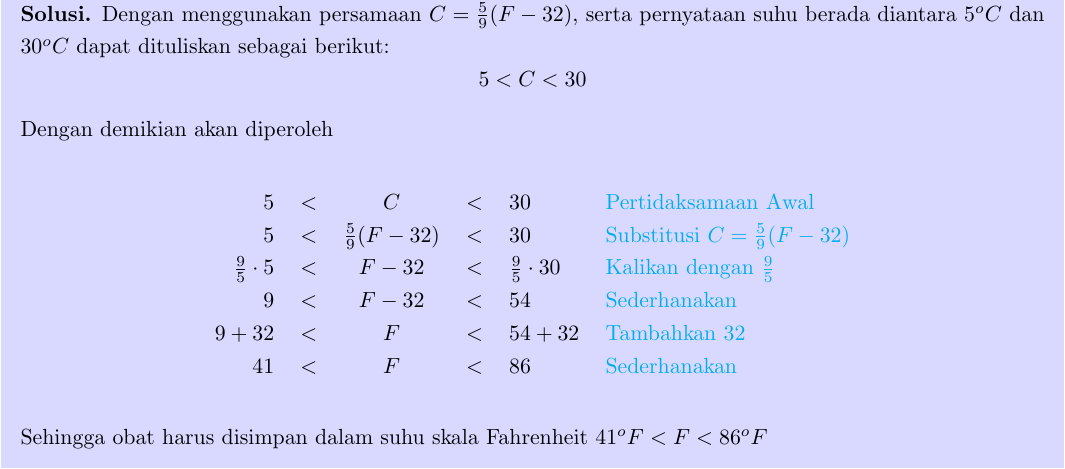
\includegraphics[width=\linewidth]{img/img17}
	\end{center}
\end{frame}

\section{Latihan Soal Pertidaksamaan}

\begin{frame}
	\frametitle{Solusi Pertidaksamaan Tak Linear}
	\begin{center}
		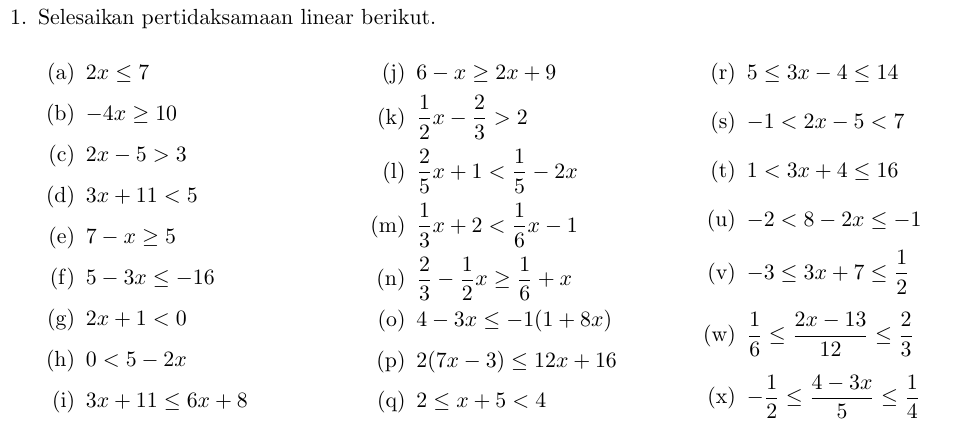
\includegraphics[width=\linewidth]{img/img18}
	\end{center}
\end{frame}

\begin{frame}
	\frametitle{Solusi Pertidaksamaan Tak Linear}
	\begin{center}
		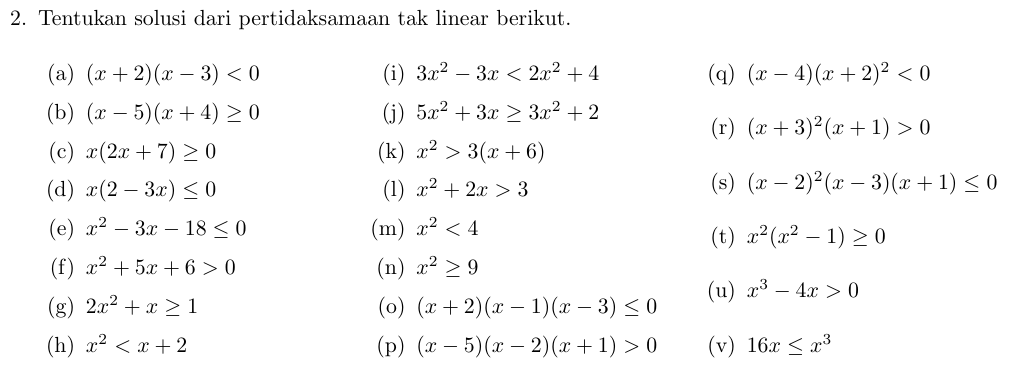
\includegraphics[width=\linewidth]{img/img19}
	\end{center}
\end{frame}

\begin{frame}
	\frametitle{Solusi Pertidaksamaan Tak Linear}
	\begin{center}
		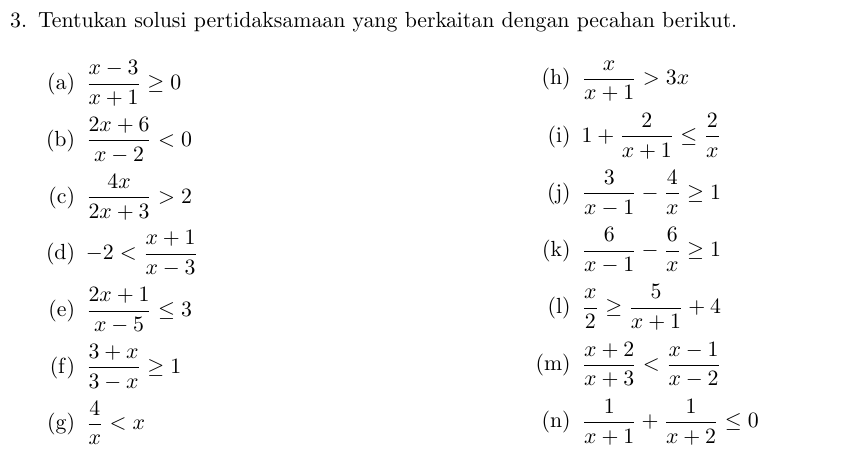
\includegraphics[width=\linewidth]{img/img20}
	\end{center}
\end{frame}

\begin{frame}
	\frametitle{Solusi Pertidaksamaan Tak Linear}
	\begin{center}
		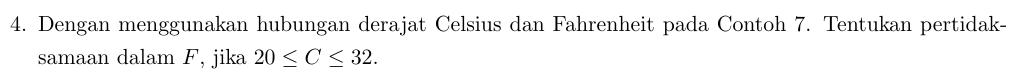
\includegraphics[width=\linewidth]{img/img21}
		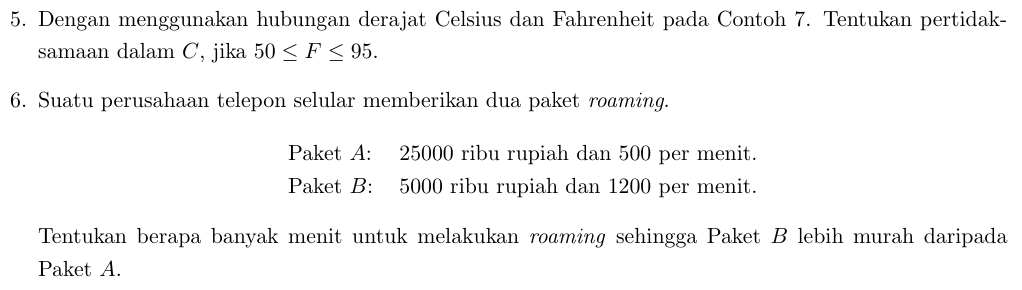
\includegraphics[width=\linewidth]{img/img22}
	\end{center}
\end{frame}

\begin{frame}
	\frametitle{Solusi Pertidaksamaan Tak Linear}
	\begin{center}
		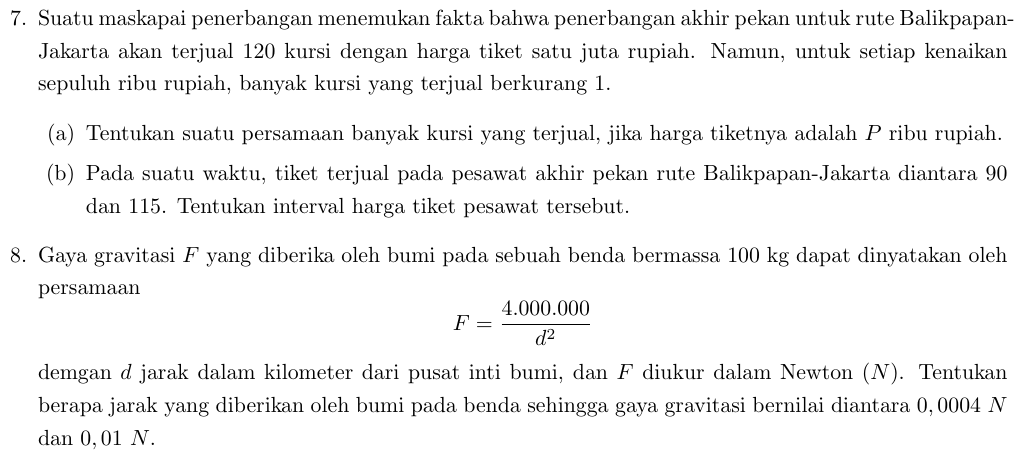
\includegraphics[width=\linewidth]{img/img23}
	\end{center}
\end{frame}

\begin{frame}
	\frametitle{Solusi Pertidaksamaan Tak Linear}
	\begin{center}
		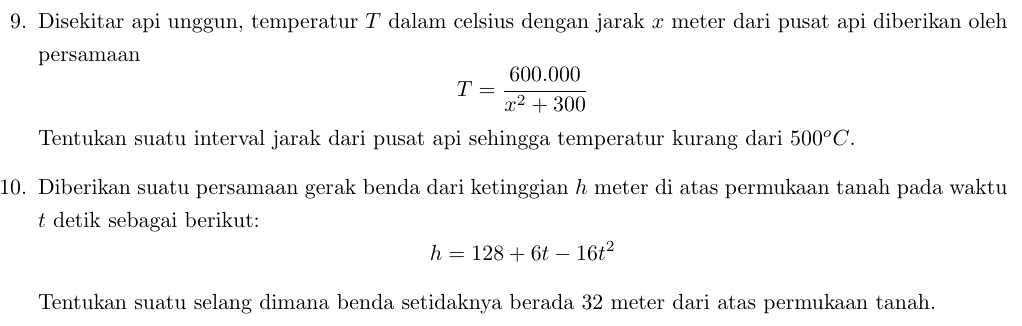
\includegraphics[width=\linewidth]{img/img24}
	\end{center}
\end{frame}

\begin{frame}
	\frametitle{Solusi Pertidaksamaan Tak Linear}
	\begin{center}
		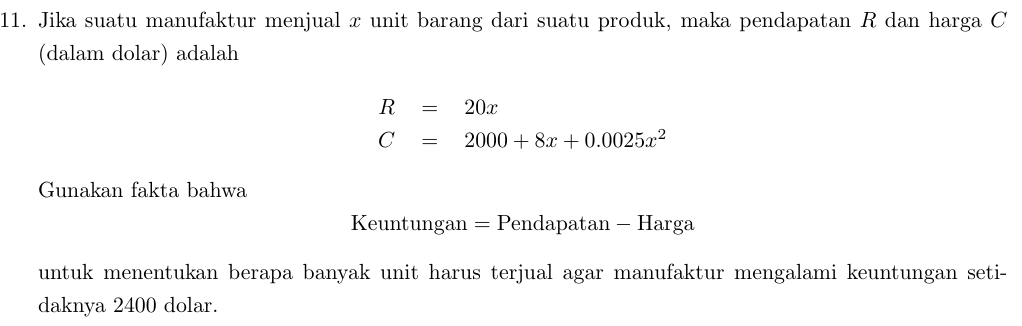
\includegraphics[width=\linewidth]{img/img25}
	\end{center}
\end{frame}

\begin{frame}
	\frametitle{Solusi Pertidaksamaan Tak Linear}
	\begin{center}
		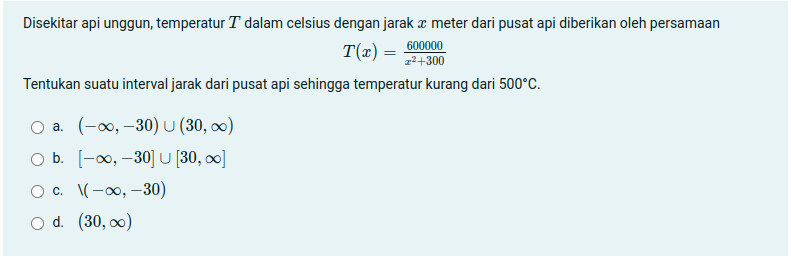
\includegraphics[width=\linewidth]{img/img26}
	\end{center}
\end{frame}

\begin{frame}
	\frametitle{Solusi Pertidaksamaan Tak Linear}
	\begin{center}
		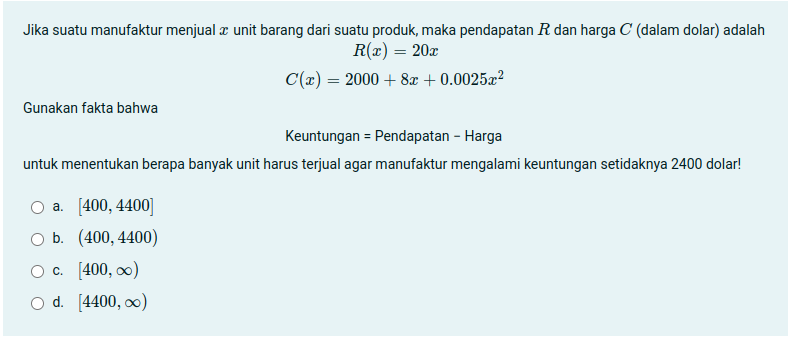
\includegraphics[width=\linewidth]{img/img27}
	\end{center}
\end{frame}


\end{document}
